\documentclass{article}
\usepackage[utf8]{inputenc}
\usepackage[T1]{fontenc}
\usepackage{graphicx}
\usepackage{hyperref}
\usepackage{geometry}
\geometry{margin=1in}

\title{HUET (Peter Daniel}
\date{Encyclopaedia Britannica (1771)}

\begin{document}
\maketitle

\section*{Historical source}
\textbf{Entry ID:} \texttt{entry-huet-peter-daniel-1327} \\
\textbf{Volume ID:} 149981670 \\
\textbf{Character Count:} 2582

\subsection*{Extracted Text}
HUET (Peter Daniel), a very learned French wri-
ter, born at Caen in Normandy, on the 8th of Re-
burry 1659. He discovered, from his infantry a
great inclination in the duty of palies literature and
the fencences, and at first applied himself to the law;
but De Carteri principles and Boehart served goes
graphy made him change his duties for thalo of phi-
hophyly, mathematics, the languages, and antiqui-
ries. His timismo is Boeharachism him delicious
of knowing him. He contened a very fact friend-
hip with him, and consomata that fared men to
Sweder. Here Chihlen would have engaged him
her teries; but the, feasible of her incumbent temper,
returned to France. All be brought with him was a
copy of a MSI, of Oregon, which he sacrificed at
Stockholm. He refuelle federal offers from Chitlina
after the billions and went to Rome, and from Ga-
tivers as far freeders. In 1670, the defining age
pointed by the king perception to the daughn, his
major, chief of the Hustic for his collegary with our
title of \_this practice\_ on the prices. It was he dust
formed the plan of the commemoration \_in often Dul.\_
\_pliant\_, and directed the execution. His intentions of
piety determined him to enter into holy orders, which
he did at the war we 44.6. Soon after this, he was per-
fetted by the long, no has abby of January and in
168s was nominated to the hillopric of Sollions, which
he exchange for the free of Armouth. After go-
verning their director ten years, his religious, and any
made about of Pontesny near Caen. His love to his
massive place determined him to the there. But that
finis coming upon him, he retired to Paris, and lodged
among the Jefuits in the \_Maifon Profiffe\_, whom he had made heys to his library. A fewer dilempper
weakened his body extremely, but was the vivacity of
his genius:' he wrote his own life in a very elegant
flyts) and died in 1721, aged 91. He was a run of
very accessible construction, 1nd of great probity, as
well as immense civilization--The following are the
titles of his principal works. 1. \_De time laungre-\_
\_values, of giving some interceptions\_. 2. An eli-
tion of Origen's comentaries on the holy Scriptures,
in Greek and Latin. 3. A travtile on the origin
of the Romanza. \_Dornedible examples, folio.\_
5. \_Sauffinese Alnetane de conocrinia romania et filais.\_
6. Of the duration of the terrestrial passifies, in
French, 7. Albility of the comments on tangica-
tion of the ancient, which has been raindicated into
English. 8. \_Demonstrate du rival and semi porti-\_
\_constitutes.\_ 9. \_Hetainas.\_ 10. Listin and Greek ver-
fen, 6.



\section*{Source record}
\begin{itemize}
\item \textbf{Dataset:} \texttt{NationalLibraryOfScotland/encyclopaedia\_britannica\_illustrated}
\item \textbf{Dataset Revision:} \texttt{309f765b1ecc83e0a7f7762e44b4a927a7555443}
\item \textbf{Page ID:} \texttt{britannica:309f765b1ecc83e0a7f7762e44b4a927a7555443:train:1327} \\
  \textbf{Filename:} \texttt{page-1327-7d41b1db21d5.jpg} \\
  \textbf{Row Index:} 1327 \\
  \textbf{SHA256:} \texttt{7d41b1db21d5e291...}
\end{itemize}

\begin{figure}[h]
\centering
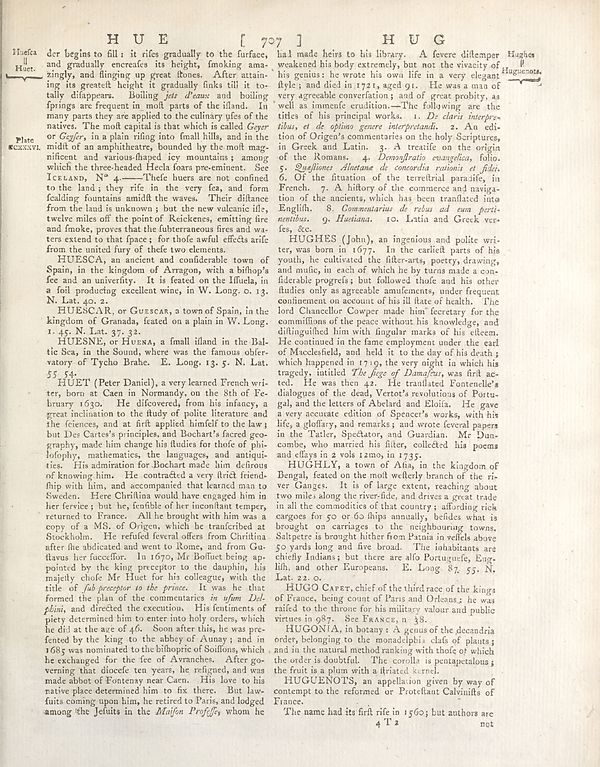
\includegraphics[width=0.85\textwidth]{../scans/page-1327-7d41b1db21d5.jpg}
\caption*{Source scan: \texttt{page-1327-7d41b1db21d5.jpg}}
\end{figure}

\end{document}
